\chapter{Pembakaran: Apa yang Diperlukan Api}\label{ch:g4:what-a-fire-needs}

Api unggun di senja hari. Api itu memerlukan kayu kering, sebatang korek
api untuk menyalakannya, dan angin yang berembus melewatinya membuatnya
tetap terang. Sejam kemudian, kayu-kayu gelondongan telah menyusut
menjadi bara yang berpijar dan abu putih, dan asap kelabu telah melayang
ke langit. Ke mana perginya kayu itu? Apa yang diperlukan api, dan apa
yang ditinggalkannya?

\begin{recall}
\omterm{def:g4:air-a-mixture-of-gases:air}{Udara} adalah campuran gas: sekitar empat perlima nitrogen dan seperlima
oksigen, dengan sedikit argon dan karbon dioksida. Nyala api mengambil
oksigen dari \omterm{def:g4:air-a-mixture-of-gases:air}{udara} di sekitarnya; lilin di bawah stoples padam ketika
oksigen yang tersisa terlalu sedikit (\cref{ch:g4:air-a-mixture-of-gases}).
\end{recall}

\begin{omfigure}
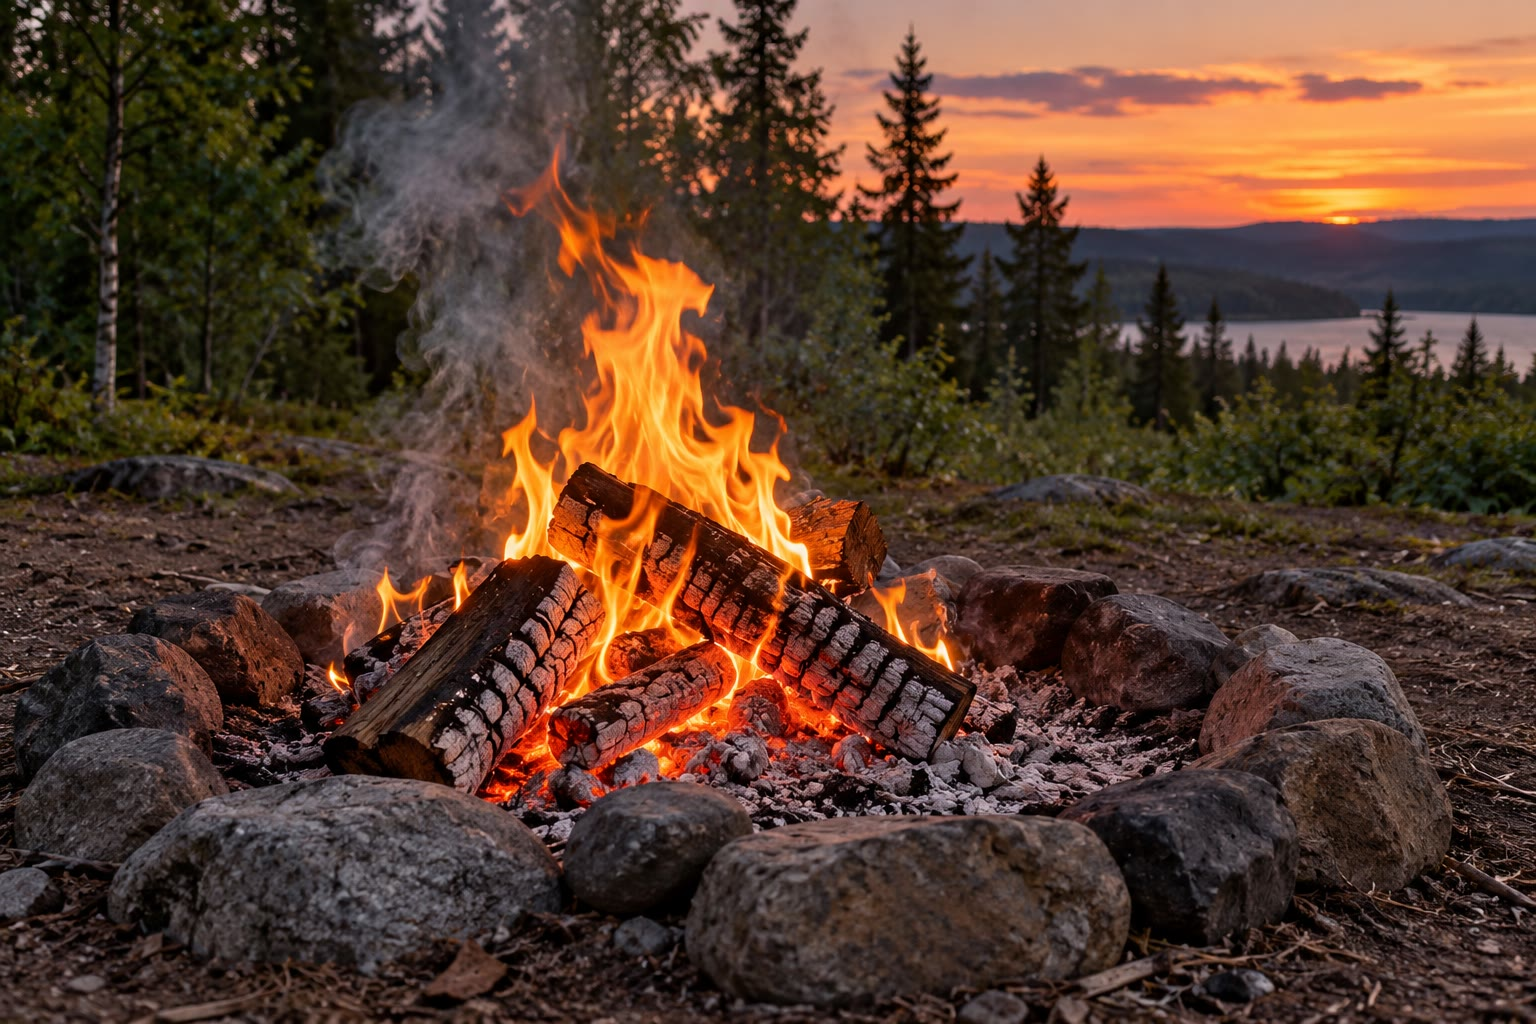
\includegraphics[width=0.6\linewidth]{images/book1/ai/g4-campfire.jpg}

{\small Api unggun: kayu, \omterm{def:g4:air-a-mixture-of-gases:air}{udara}, dan korek api --- lalu sesudahnya abu
dan asap.}
\end{omfigure}

\section{Bahan bakar}

\begin{definition}[Bahan bakar]\label{def:g4:what-a-fire-needs:fuel}
Yang disebut \emph{bahan bakar}\index{bahan bakar} adalah bahan yang
dapat \omterm{def:g4:what-a-fire-needs:burning}{terbakar} serta mengeluarkan panas dan cahaya: kayu, kertas,
batu bara, lilin, gas kompor, bensin, minyak tanah.
\end{definition}

\begin{example}[Bahan bakar padat, cair, dan gas]\label{ex:g4:what-a-fire-needs:fuels}
Kayu, kertas, batu bara, dan lilin adalah \omterm{def:g4:what-a-fire-needs:fuel}{bahan bakar} padat. Bensin dan
minyak tanah adalah \omterm{def:g4:what-a-fire-needs:fuel}{bahan bakar} cair. Gas kompor dapur dan gas di dalam
korek api gas adalah \omterm{def:g4:what-a-fire-needs:fuel}{bahan bakar} gas.
\end{example}

\begin{remark}[Tidak semua benda dapat terbakar]\label{rem:g4:what-a-fire-needs:not}
Batu, pasir, kaca, dan air tidak dapat \omterm{def:g4:what-a-fire-needs:burning}{terbakar}: semuanya bukan \omterm{def:g4:what-a-fire-needs:fuel}{bahan
bakar}. Karena itulah perapian dibangun dari batu atau bata, dan pasir
serta air dipakai untuk memadamkan api.
\end{remark}

\section{Segitiga api}

\begin{definition}[Segitiga api]\label{def:g4:what-a-fire-needs:fire-triangle}
Api memerlukan tiga hal sekaligus: \omterm{def:g4:what-a-fire-needs:fuel}{bahan bakar}, oksigen dari \omterm{def:g4:air-a-mixture-of-gases:air}{udara}, dan
panas untuk menyalakannya. Ketiga hal itu digambar sebagai tiga sisi
sebuah segitiga, yaitu \emph{segitiga api}\index{segitiga api}. Jika
salah satu sisinya tidak ada, tidak ada api.
\end{definition}

\begin{omfigure}
\begin{tikzpicture}[font=\small]
  \coordinate (A) at (0,0); \coordinate (B) at (5,0); \coordinate (C) at (2.5,4.1);
  \draw[line width=3pt, brown!70!black] (A) -- (B);
  \draw[line width=3pt, omDef] (B) -- (C);
  \draw[line width=3pt, red!75!black] (C) -- (A);
  \node[below=4pt, font=\small\bfseries, brown!60!black] at (2.5,0) {bahan bakar};
  \node[right=4pt, font=\small\bfseries, omDef] at (3.75,2.05) {oksigen (dari udara)};
  \node[left=4pt, font=\small\bfseries, red!75!black] at (1.25,2.05) {panas (penyulut)};
  % a flame in the middle
  \fill[orange!80] (2.5,0.55) .. controls (1.95,1.15) and (2.35,1.75) .. (2.55,2.3)
    .. controls (2.75,1.75) and (3.05,1.15) .. (2.5,0.55);
  \fill[yellow!80] (2.5,0.7) .. controls (2.25,1.05) and (2.4,1.35) .. (2.52,1.65)
    .. controls (2.62,1.35) and (2.75,1.05) .. (2.5,0.7);
\end{tikzpicture}

{\small \omterm{def:g4:what-a-fire-needs:fire-triangle}{Segitiga api}: \omterm{def:g4:what-a-fire-needs:fuel}{bahan bakar}, oksigen, dan panas, ketiganya bersama-sama.}
\end{omfigure}

\begin{example}[Menyalakan korek api]\label{ex:g4:what-a-fire-needs:match}
Kepala korek api digosokkan ke sisi kotaknya. Gosokan itu memanaskannya
cukup untuk membuatnya mulai \omterm{def:g4:what-a-fire-needs:burning}{terbakar}: itulah sisi panas pada segitiga.
Kayu batang korek itu adalah \omterm{def:g4:what-a-fire-needs:fuel}{bahan bakarnya}, dan \omterm{def:g4:air-a-mixture-of-gases:air}{udara} membawa
oksigennya.
\end{example}

\begin{example}[Meniup bara]\label{ex:g4:what-a-fire-needs:embers}
Bara berpijar yang tampak hampir padam menyala lagi ketika seseorang
meniupnya: tiupan itu membawa lebih banyak \omterm{def:g4:air-a-mixture-of-gases:air}{udara}, jadi lebih banyak
oksigen, ke \omterm{def:g4:what-a-fire-needs:fuel}{bahan bakar} yang masih panas.
\end{example}

\section{Pembakaran menghasilkan zat baru}

\begin{definition}[Terbakar dan pembakaran]\label{def:g4:what-a-fire-needs:burning}
Sebuah \omterm{def:g4:what-a-fire-needs:fuel}{bahan bakar} \emph{terbakar}\index{terbakar} ketika ia mengambil
oksigen dari \omterm{def:g4:air-a-mixture-of-gases:air}{udara} serta mengeluarkan panas dan cahaya. Para ahli kimia
menyebut peristiwa itu \emph{pembakaran}\index{pembakaran}. Selama
pembakaran, \omterm{def:g4:what-a-fire-needs:fuel}{bahan bakar} dan oksigen terpakai habis, dan muncul zat-zat
baru: asap, abu, karbon dioksida, dan uap air.
\end{definition}

\begin{proposition}[Pembakaran tidak dapat dibatalkan]\label{prop:g4:what-a-fire-needs:new}
Abu dan asap api tidak berubah kembali menjadi kayu, selama apa pun kita
menunggu. \omterm{def:g4:what-a-fire-needs:burning}{Pembakaran} menghasilkan zat-zat baru yang sebelumnya tidak
ada; \omterm{def:g4:what-a-fire-needs:fuel}{bahan bakarnya} hilang untuk selamanya.
\end{proposition}

\begin{inthelab}[Gelas dingin di atas lilin]
Guru memegang sebuah gelas kimia yang dingin dan kering secara terbalik
sesaat di atas nyala lilin. Bagian dalam gelas itu berembun oleh
titik-titik air yang sangat kecil: uap air yang dihasilkan lilin yang
\omterm{def:g4:what-a-fire-needs:burning}{terbakar} telah kembali menjadi cairan pada kaca yang dingin. Lilin yang
\omterm{def:g4:what-a-fire-needs:burning}{terbakar} menghasilkan air, dan juga karbon dioksida, yang dapat
dideteksi dengan sebuah uji yang akan kita temui di bab berikutnya.
\end{inthelab}

\begin{omfigure}
\begin{tikzpicture}[font=\small, scale=1.3]
  % candle
  \fill[white, draw=black!50] (-0.25,0) rectangle (0.25,1.2);
  \draw[black!70] (0,1.2) -- (0,1.33);
  \fill[orange!85] (0,1.3) .. controls (-0.16,1.5) and (-0.06,1.75) .. (0,1.95)
    .. controls (0.06,1.75) and (0.16,1.5) .. (0,1.3);
  \fill[yellow!85] (0,1.36) .. controls (-0.08,1.5) and (-0.03,1.62) .. (0,1.72)
    .. controls (0.03,1.62) and (0.08,1.5) .. (0,1.36);
  % upturned cold beaker above
  \pic[transform shape, rotate=180] at (0,4.3) {beaker={0}{white}};
  \foreach \x/\y in {-0.6/3.9,-0.45/4.1,-0.2/3.95,0.1/4.15,0.35/3.9,0.6/4.05,
                     -0.7/3.5,0.7/3.4,-0.72/3.0,0.72/2.9}
    \fill[omDef!55] (\x,\y) circle (0.035);
  \draw[<-, omProp, thick] (0.68,3.95) -- (2.0,4.2) node[right, text=black]
    {titik-titik air};
  \draw[<-, omProp, thick] (0.85,3.2) -- (2.0,3.3) node[right, text=black]
    {gelas dingin, terbalik};
  \draw[<-, omProp, thick] (0.15,1.7) -- (2.0,1.9) node[right, text=black]
    {nyala api: lilin terbakar};
  \draw[<-, omProp, thick] (0.3,0.6) -- (2.0,0.7) node[right, text=black]
    {lilin: bahan bakarnya};
\end{tikzpicture}

{\small Gelas dingin yang dipegang di atas lilin berembun: lilin yang
\omterm{def:g4:what-a-fire-needs:burning}{terbakar} menghasilkan uap air.}
\end{omfigure}

\begin{example}[Menjadi apa sebatang kayu gelondongan]\label{ex:g4:what-a-fire-needs:log}
Kayu gelondongan seberat beberapa kilogram \omterm{def:g4:what-a-fire-needs:burning}{terbakar} habis menjadi
setumpuk kecil abu. Sebagian besar kayunya tidak lenyap: bersama oksigen
dari \omterm{def:g4:air-a-mixture-of-gases:air}{udara}, kayu itu telah menjadi asap, karbon dioksida, dan uap air,
yang berupa gas dan melayang ke langit.
\end{example}

\section{Memadamkan api}

\begin{method}[Memadamkan api: hilangkan satu sisi]\label{met:g4:what-a-fire-needs:out}
Untuk memadamkan api, hilangkan satu sisi \omterm{def:g4:what-a-fire-needs:fire-triangle}{segitiga api}:
\begin{itemize}
  \item \textbf{hilangkan oksigennya}: tutup api dengan selimut api,
        tutup panci, atau pasir, sehingga \omterm{def:g4:air-a-mixture-of-gases:air}{udara} tidak dapat mencapainya;
  \item \textbf{hilangkan panasnya}: siram kayu atau kertas yang
        \omterm{def:g4:what-a-fire-needs:burning}{terbakar} dengan air, yang mendinginkannya sampai di bawah titik
        tempat ia dapat \omterm{def:g4:what-a-fire-needs:burning}{terbakar};
  \item \textbf{hilangkan \omterm{def:g4:what-a-fire-needs:fuel}{bahan bakarnya}}: tutup keran gas, atau
        bersihkan tumbuhan kering di sekitar kebakaran hutan.
\end{itemize}
\end{method}

\begin{omfigure}
\begin{tikzpicture}[font=\small, scale=0.7]
  \foreach \k/\lab/\side in {0/{selimut: tanpa oksigen}/1, 1/{air: tanpa panas}/2,
                              2/{gas dimatikan: tanpa bahan bakar}/0} {
    \begin{scope}[xshift=\k*6.2cm]
      \coordinate (A) at (0,0); \coordinate (B) at (4,0); \coordinate (C) at (2,3.3);
      \pgfmathsetmacro\oa{\side==0 ? 0.2 : 1}
      \pgfmathsetmacro\ob{\side==1 ? 0.2 : 1}
      \pgfmathsetmacro\oc{\side==2 ? 0.2 : 1}
      \draw[line width=2.5pt, brown!70!black, opacity=\oa] (A) -- (B);
      \draw[line width=2.5pt, omDef, opacity=\ob] (B) -- (C);
      \draw[line width=2.5pt, red!75!black, opacity=\oc] (C) -- (A);
      \ifnum\side=0 \draw[line width=1.4pt, black] (1.6,-0.4) -- (2.4,0.4) (1.6,0.4) -- (2.4,-0.4);\fi
      \ifnum\side=1 \draw[line width=1.4pt, black] (2.6,1.25) -- (3.4,2.05) (2.6,2.05) -- (3.4,1.25);\fi
      \ifnum\side=2 \draw[line width=1.4pt, black] (0.6,1.25) -- (1.4,2.05) (0.6,2.05) -- (1.4,1.25);\fi
      \node[align=center, anchor=north] at (2,-0.6) {\lab};
    \end{scope}
  }
\end{tikzpicture}

{\small Tiga cara memadamkan api, masing-masing menghilangkan satu sisi
segitiga (yang dicoret): oksigen, panas, atau \omterm{def:g4:what-a-fire-needs:fuel}{bahan bakar}.}
\end{omfigure}

\begin{omfigure}
\begin{minipage}[t]{0.48\linewidth}\centering
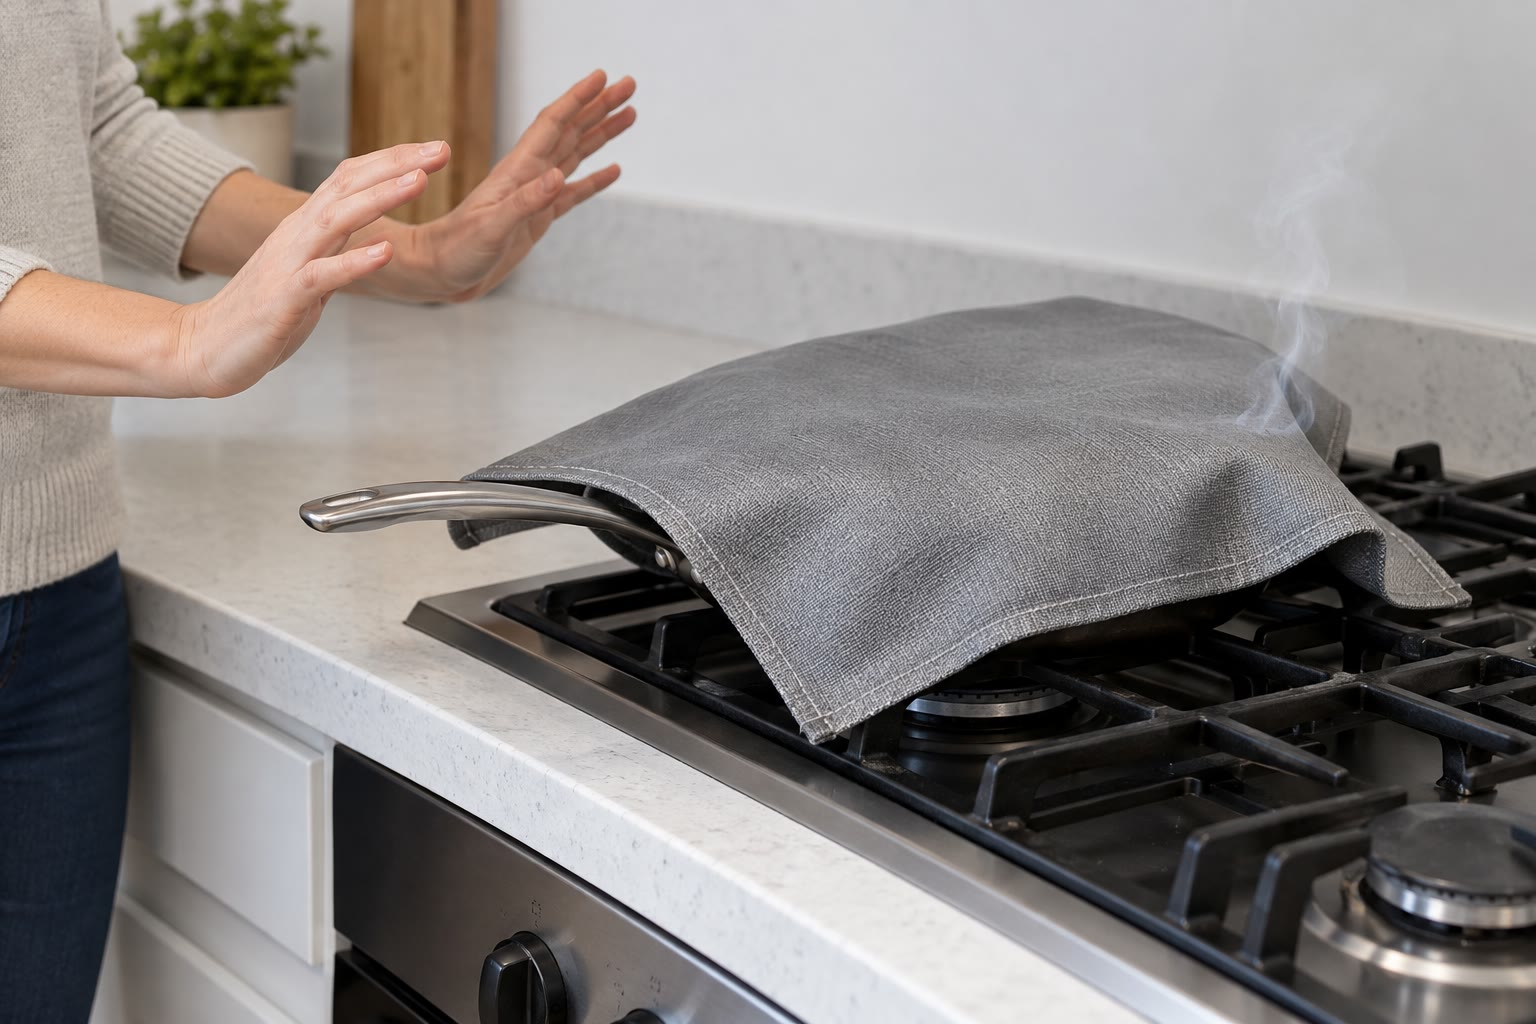
\includegraphics[width=\linewidth,height=4.6cm,keepaspectratio]{images/book1/ai/g4-fire-blanket.jpg}

{\small Selimut api di atas wajan: \omterm{def:g4:air-a-mixture-of-gases:air}{udara} tidak dapat lagi mencapai
api.}
\end{minipage}\hfill
\begin{minipage}[t]{0.48\linewidth}\centering
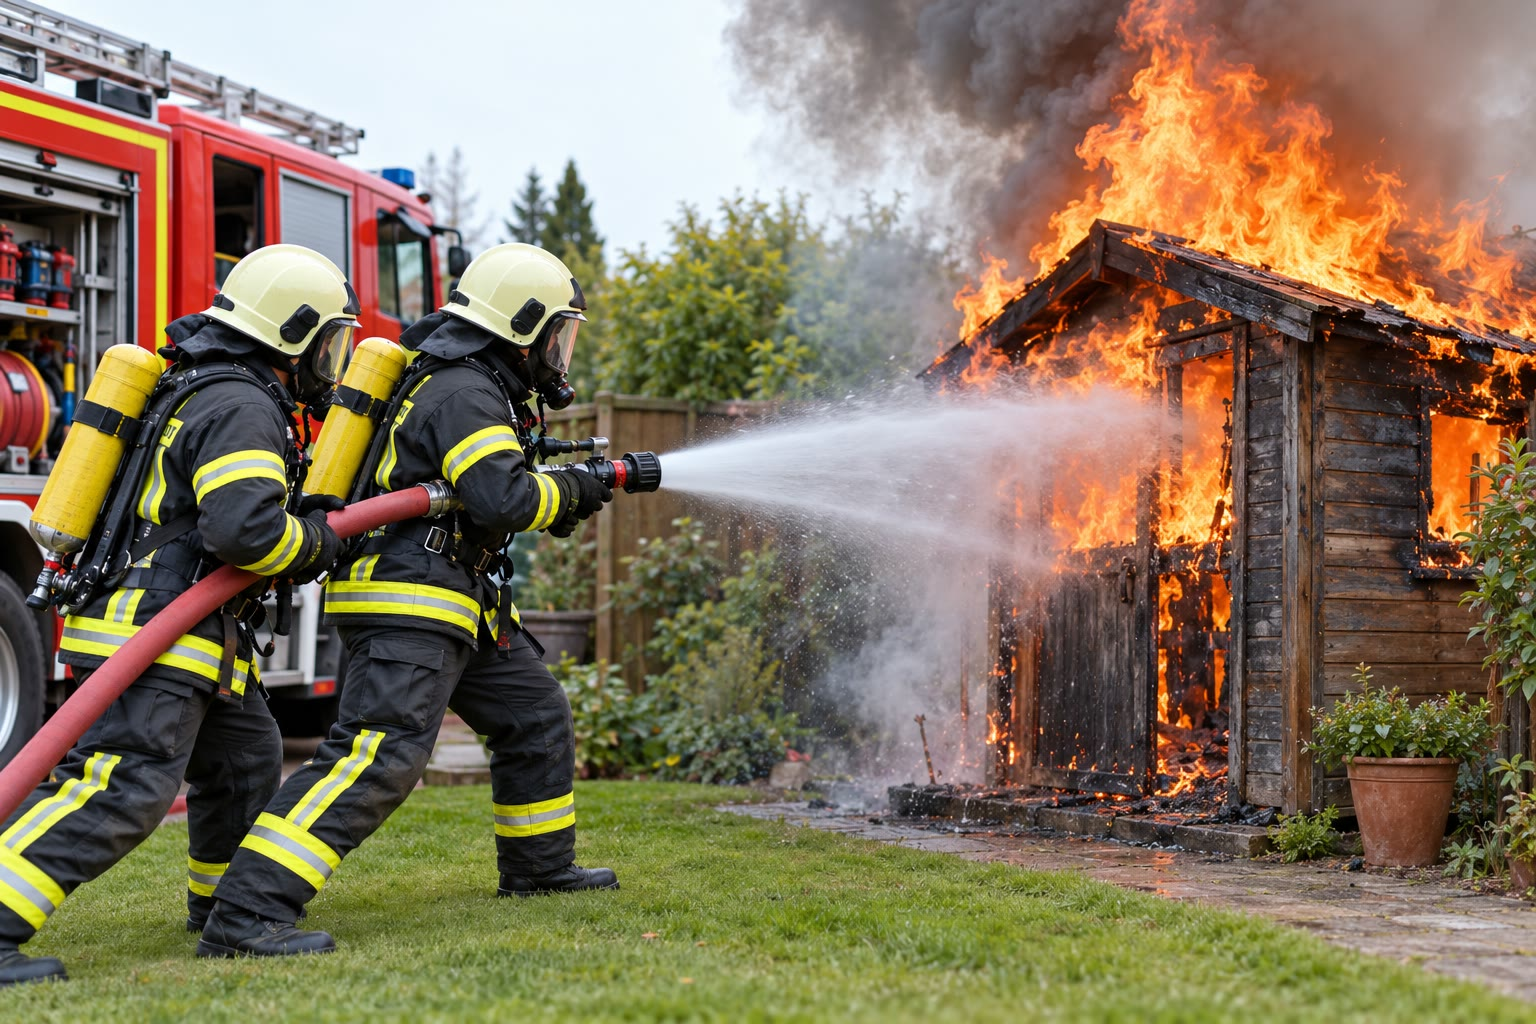
\includegraphics[width=\linewidth,height=4.6cm,keepaspectratio]{images/book1/ai/g4-firefighters.jpg}

{\small Petugas pemadam kebakaran menyemprotkan air untuk mendinginkan
gudang yang \omterm{def:g4:what-a-fire-needs:burning}{terbakar}.}
\end{minipage}
\end{omfigure}

\section{Keselamatan dari kebakaran}

\begin{remark}[Jangan pernah menyiram minyak yang terbakar dengan air]\label{rem:g4:what-a-fire-needs:oil}
Jika minyak di wajan \omterm{def:g4:what-a-fire-needs:burning}{terbakar}, tidak seorang pun boleh menyiramnya
dengan air: air langsung mendidih di bawah minyak dan melontarkan minyak
yang \omterm{def:g4:what-a-fire-needs:burning}{terbakar} keluar dari wajan. Kompor gas atau kompor listriknya
dimatikan dan wajannya ditutup dengan tutup panci atau selimut api, oleh
orang dewasa.
\end{remark}

\begin{safety}{\ghs{GHS02}\ghs{GHS04}}
% ledger: ghs:butane
Gas di dalam korek api gas atau tabung gas kemah adalah butana.
Piktogram nyala apinya (GHS02) berarti: sangat mudah menyala, jauhkan
dari api dan percikan api. Piktogram tabung gas (GHS04) berarti: gas
yang disimpan di bawah tekanan.
\end{safety}

\begin{proposition}[Yang harus dilakukan jika terjadi kebakaran]\label{prop:g4:what-a-fire-needs:safety}
Asap adalah bahaya pertama dalam kebakaran: asap itu panas,
menyembunyikan jalan keluar, dan beracun bila dihirup. Alarm asap di
langit-langit berbunyi keras begitu asap mencapainya. Jika terjadi
kebakaran: keluarlah, tetap merunduk di bawah asap, tutup pintu di
belakangmu, dan teleponlah pemadam kebakaran dari luar. Jangan pernah
masuk kembali.
\end{proposition}

\begin{omfigure}
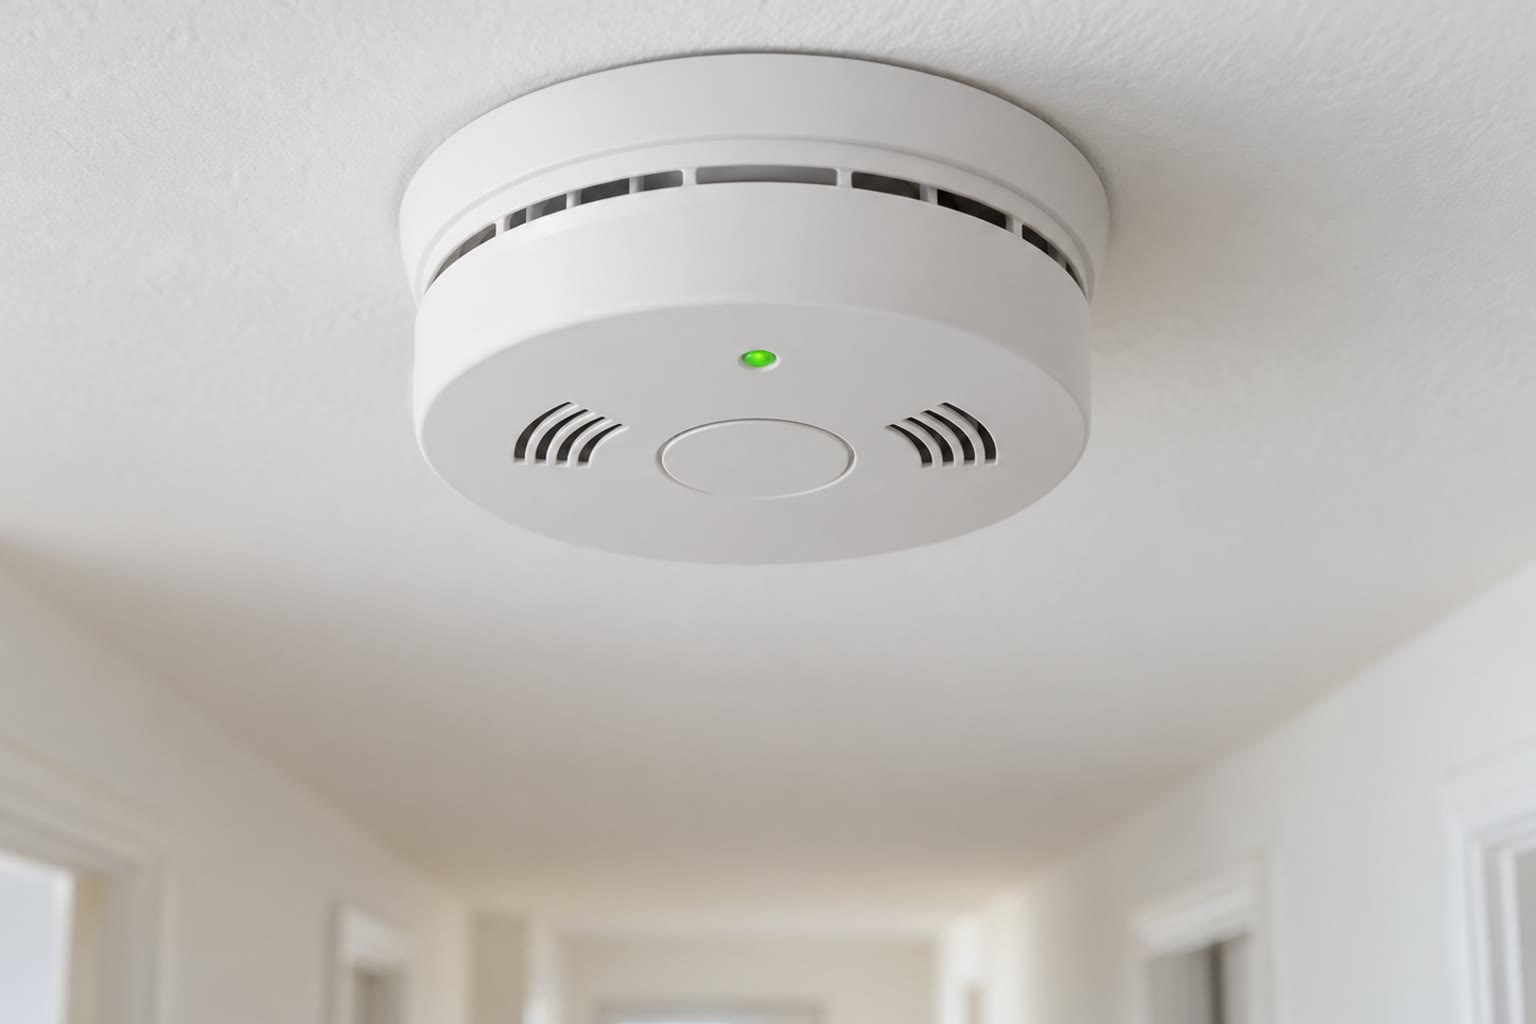
\includegraphics[width=0.42\linewidth]{images/book1/ai/g4-smoke-alarm.jpg}

{\small Alarm asap: alarm itu berbunyi begitu asap mencapainya.}
\end{omfigure}

\section{Latihan}

\begin{exercise}[$\star$]\label{exo:g4:what-a-fire-needs:1}
Sebutkan ketiga sisi \omterm{def:g4:what-a-fire-needs:fire-triangle}{segitiga api}.
\end{exercise}

\begin{exercise}[$\star$]\label{exo:g4:what-a-fire-needs:2}
Manakah yang merupakan \omterm{def:g4:what-a-fire-needs:fuel}{bahan bakar}: kayu, pasir, lilin, kaca, bensin,
air, kertas?
\end{exercise}

\begin{exercise}[$\star$]\label{exo:g4:what-a-fire-needs:3}
Sebuah selimut api dilemparkan ke atas api kecil. Sisi \omterm{def:g4:what-a-fire-needs:fire-triangle}{segitiga api}
mana yang dihilangkannya?
\end{exercise}

\begin{exercise}[$\star$]\label{exo:g4:what-a-fire-needs:4}
Petugas pemadam kebakaran menyemprotkan air ke gudang yang \omterm{def:g4:what-a-fire-needs:burning}{terbakar}.
Sisi \omterm{def:g4:what-a-fire-needs:fire-triangle}{segitiga api} mana yang dihilangkan oleh air itu?
\end{exercise}

\begin{exercise}[$\star$]\label{exo:g4:what-a-fire-needs:5}
Sebutkan tiga zat baru yang dihasilkan ketika kayu \omterm{def:g4:what-a-fire-needs:burning}{terbakar}.
\end{exercise}

\begin{exercise}[$\star$]\label{exo:g4:what-a-fire-needs:6}
Mengapa meniup bara yang berpijar membuatnya berkobar lagi?
\end{exercise}

\begin{exercise}[$\star$]\label{exo:g4:what-a-fire-needs:7}
Gelas dingin yang dipegang di atas lilin berembun. Zat baru apa yang
telah dihasilkan lilin itu?
\end{exercise}

\begin{exercise}[$\star$]\label{exo:g4:what-a-fire-needs:8}
Apa yang harus kamu lakukan pertama kali jika alarm asap berbunyi dan
kamu melihat asap?
\end{exercise}

\begin{exercise}[$\star$]\label{exo:g4:what-a-fire-needs:9}
Lihatlah gambar dengan tiga segitiga kecil. Sisi mana yang dicoret
ketika gas dimatikan?
\end{exercise}

\begin{exercise}[$\star\star$]\label{exo:g4:what-a-fire-needs:10}
Untuk menghentikan kebakaran hutan, petugas pemadam kebakaran kadang
menebang sejalur lebar pepohonan di depan api. Sisi \omterm{def:g4:what-a-fire-needs:fire-triangle}{segitiga api} mana
yang mereka hilangkan?
\end{exercise}

\begin{exercise}[$\star\star$]\label{exo:g4:what-a-fire-needs:11}
Sebatang kayu gelondongan jauh lebih berat daripada abunya. Apakah
sebagian kayu itu lenyap? Jelaskan ke mana perginya.
\end{exercise}
